\documentclass[12pt,letterpaper]{exam}
\usepackage[lmargin=1in,rmargin=1in,tmargin=1in,bmargin=1in]{geometry}
\usepackage{../style/exams}

% -------------------
% Course & Exam Information
% -------------------
\newcommand{\course}{MATH 115: Final Exam}
\newcommand{\term}{Fall --- 2024}
\newcommand{\examdate}{12/11/2024}
\newcommand{\timelimit}{150 Minutes}

\setbool{hideans}{true} % Student: True; Instructor: False

\usepackage{multicol}
\newenvironment{2enumerate}{%
\begin{enumerate}[(a)]
\begin{multicols}{2}
}{%
\end{multicols}
\end{enumerate}
}

% -------------------
% Content
% -------------------
\begin{document}

\examtitle
\instructions{Write your name on the appropriate line on the exam cover sheet. This exam contains \numpages\ pages (including this cover page) and \numquestions\ questions. Check that you have every page of the exam. Answer the questions in the spaces provided on the question sheets. Be sure to answer every part of each question and show all your work. If you run out of room for an answer, continue on the back of the page --- being sure to indicate the problem number.} 
\scores
\bottomline
\newpage

% Poem
\phantom{.} \vfill
	\begin{table}[h]
	\centering
	\begin{tabular}{l}
	{\itshape 'Twas the night before Christmas, up at the Pole,} \\
	{\itshape Santa was frazzled---he'd lost all control!} \\
	{\itshape The reindeer were restless, the sleight off its track,} \\
	{\itshape And the toy distribution? A logistical smack!} \\
	\\
	{\itshape Santa scratched his beard, eyes weary and red,} \\
	{\itshape ``The math here is tricky. I'm in over my head!} \\
	{\itshape The children are waiting, and I need to take flight.} \\
	{\itshape I need a Precalculus wizard to save Christmas tonight!''}
	\end{tabular}
	\end{table}
\phantom{.} \vfill 

% -------------------
% Questions
% -------------------
\begin{questions}

% Question 1
\newpage
\question[10] {\itshape Santa's lost in the sky, the directions aren't right, \par \phantom{(XX) points)} ``Help me compute these angles to save Christmas night!”} \par\vspace{0.3cm}

Below is a blank unit circle. Fill in each blank entry. The outside blank points should be the point on the unit circle. The innermost blank inside the unit circle should be the angle measure in degrees while the outer blank inside the unit circle is the angle measure in radians. 
	\[
	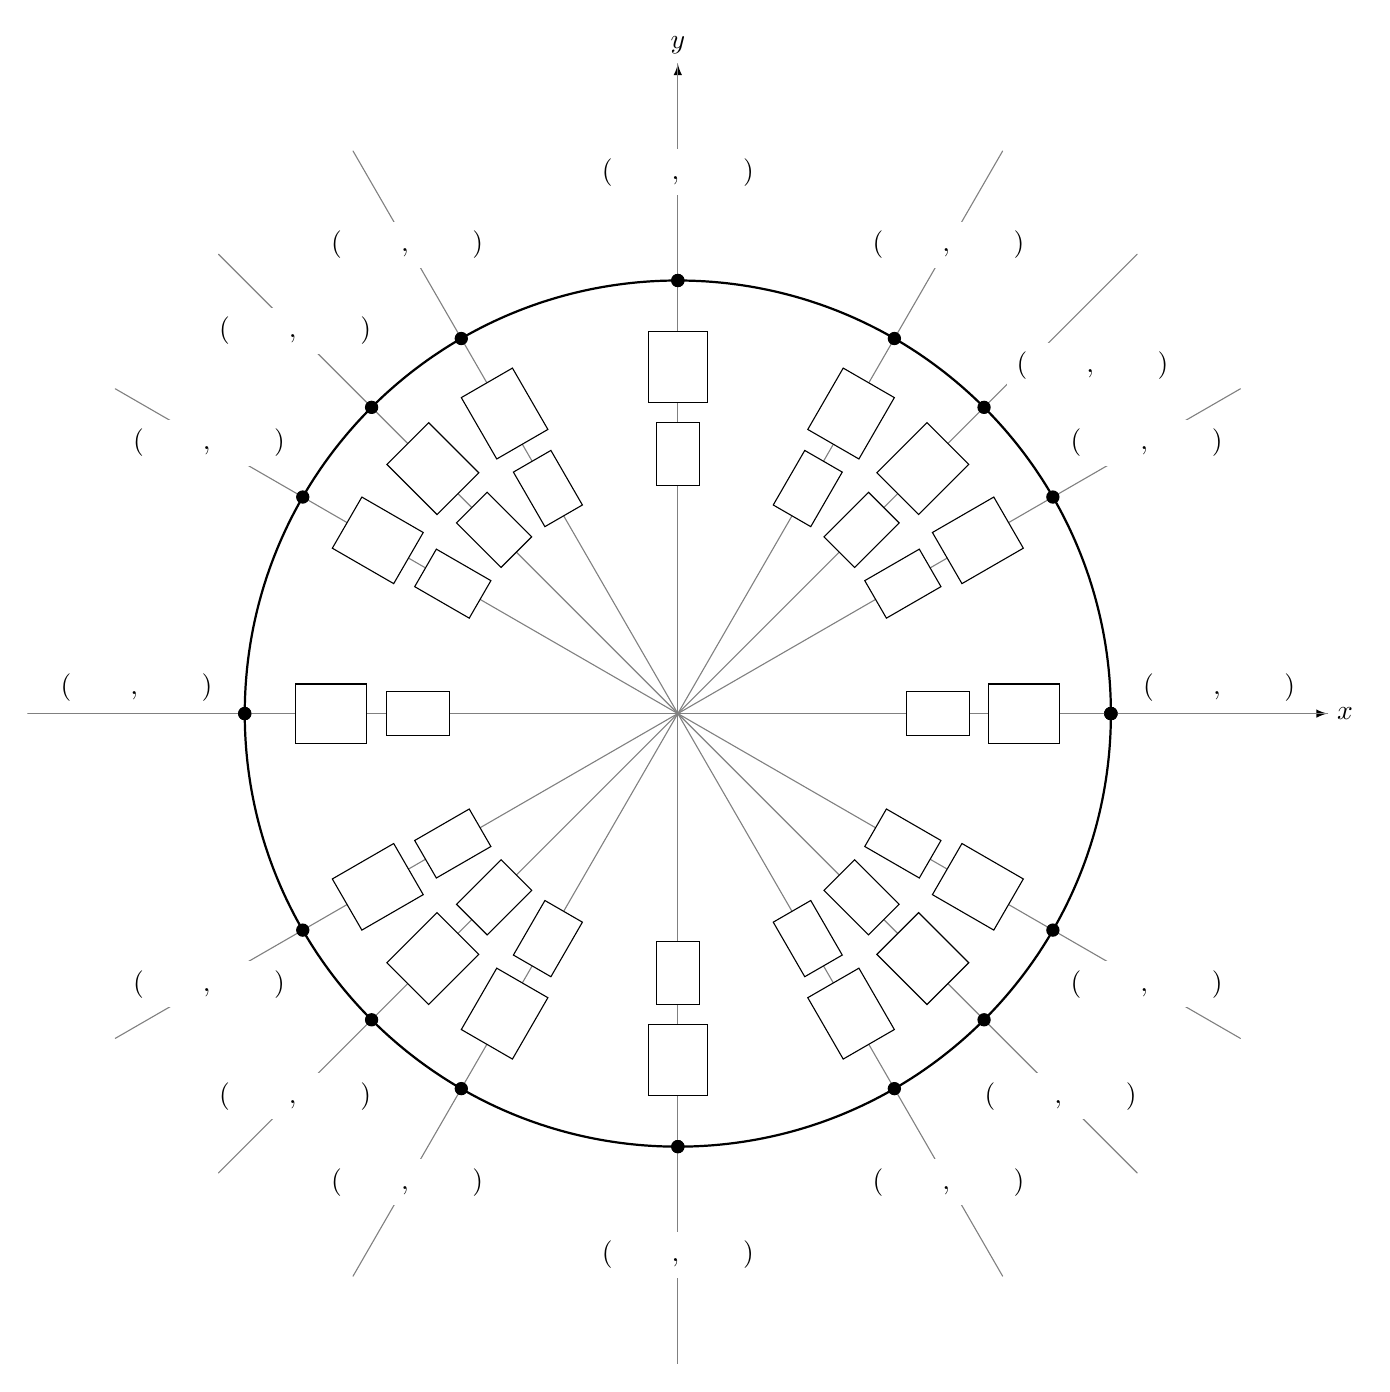
\begin{tikzpicture}[scale=5.5,cap=round,>=latex]

	% Coordinate Axes 
        \draw[->] (-1.5cm ,0cm) -- (1.5cm, 0cm) node[right, fill= white] {$x$};
        \draw[->] (0cm, -1.5cm) -- (0cm, 1.5cm) node[above, fill= white] {$y$};

	% Unit Circle
        \draw[thick] (0cm,0cm) circle(1cm);

	% '30-type' Angles
        \foreach \x in {0,30,...,360} {
                % Line from Center to Point
                \draw[gray] (0cm, 0cm) -- (\x:1.5cm);
                % Dot at Each Points
                \filldraw[black] (\x:1cm) circle(0.4pt);
                % Angles in Degrees
		\draw node[draw, fill= white, shape= rectangle, minimum height= 0.55cm, minimum width= 0.8cm, anchor= center, rotate= \x] at (\x:0.6cm) {};
		% Angle in Radians
		\draw node[draw, fill= white, shape= rectangle, minimum height= 0.75cm, minimum width= 0.9cm, anchor= center, rotate= \x] at (\x:0.8cm) {};
	}
	
	% '45-type' Angles			
	\foreach \x in {0,45,...,360} {
		% Line from Center to Point		
		\draw[gray] (0cm, 0cm) -- (\x:1.5cm);
                % Dot at Each Points			
		\filldraw[black] (\x:1cm) circle(0.4pt);
                % Angles in Degrees
		\draw node[draw, fill= white, shape= rectangle, minimum height= 0.55cm, minimum width= 0.8cm, anchor= center, rotate= \x] at (\x:0.6cm) {};
		% Angle in Radians
		\draw node[draw, fill= white, shape= rectangle, minimum height= 0.75cm, minimum width= 0.9cm, anchor= center, rotate= \x] at (\x:0.8cm) {};
	}
		
	% Horizontal/Vertical Point Placement (Better in this Format)
        \draw (-1.25cm,0cm) node[above=1pt] {$(\hspace{.75cm},\hspace{.75cm})$}
	(1.25cm,0cm)  node[above=1pt] {$(\hspace{.75cm},\hspace{.75cm})$}
	(0cm,-1.25cm) node[fill=white] {$(\hspace{.75cm},\hspace{.75cm})$}
	(0cm,1.25cm)  node[fill=white] {$(\hspace{.75cm},\hspace{.75cm})$};
	
	% Point Placement (Inner)			
	\foreach \x/\xtext/\y in {
		% Q1
		30/\hspace{.75cm}/\hspace{.75cm},
		40/\hspace{.75cm}/\hspace{.75cm},
		60/\hspace{.75cm}/\hspace{.75cm},
		% Q2
		150/\hspace{.75cm}/\hspace{.75cm},
		135/\hspace{.75cm}/\hspace{.75cm},
		120/\hspace{.75cm}/\hspace{.75cm},
		% Q3
		210/\hspace{.75cm}/\hspace{.75cm},
		225/\hspace{.75cm}/\hspace{.75cm},
		240/\hspace{.75cm}/\hspace{.75cm},
		% Q4
		330/\hspace{.75cm}/\hspace{.75cm},
		315/\hspace{.75cm}/\hspace{.75cm},
		300/\hspace{.75cm}/\hspace{.75cm}}
		\draw (\x:1.25cm) node[fill=white] {$\left(\xtext,\y\right)$};

	\end{tikzpicture}
	\]



% Question 2
\newpage
\question[15] {\itshape Santa's sleigh is in trouble, the tech's gone awry, \par \phantom{(XX points)} ``Help me crunch these numbers, or we'll fall out of the sky!”} \par\vspace{0.3cm}

Find the exact value for each of the following: \par\vspace{0.3cm}
	\begin{2enumerate}
	\item $\log_3 \!\left( \dfrac{1}{27} \right)=$ \par\vspace{1.8cm}
	\item $\tan(135^\circ)=$ \par\vspace{1.8cm}
	\item $\log_5 \left( \sqrt[4]{5} \right)=$ \par\vspace{1.8cm}
	\item $\cos \!\left( \dfrac{5\pi}{3} \right)=$ \par\vspace{1.8cm}
	\item $\tan^{-1}(`\infty\text{'})=$ \par\vspace{1.8cm}
	\item $\log_\pi (1)=$ \par\vspace{1.8cm}
	\item $\sin \!\left(-\dfrac{2\pi}{3} \right)=$ \par\vspace{1.8cm}
	\item $\log_8 (4)=$ \par\vspace{1.8cm}
	\item $\sec(150^\circ)=$ \par\vspace{1.8cm}
	\item $\arcsin(0.5)=$ \par\vspace{1.8cm}
	\item $\log_{\sqrt{2}} (4)=$ \par\vspace{1.8cm}
	\item $\ln(\sqrt{e^3})=$ \par\vspace{1.8cm}
	\item $\arccos(-1)=$ \par\vspace{1.8cm}
	\item $\csc \!\left( -\dfrac{\pi}{6} \right)=$ \par\vspace{1.8cm}
	\item $\log_7(7^{\sqrt{3}})=$ \par\vspace{1.8cm}
	\item $5^{\log_5(0.71)}=$ \par\vspace{1.8cm}
	\end{2enumerate}



% Question 3
\newpage
\question[10] {\itshape Santa's sleigh is unsteady, the flight path's complex, \par \phantom{(XX points)} ``Help me save Christmas---just find me the vertex!''} \par\vspace{0.3cm}

Consider the function $f(x)= x^2 + 8x + 13$.
	\begin{enumerate}[(a)]
	\item Find the vertex form of $f(x)$. \vfill
	\item Use (a) to identify the vertex for $f(x)$. \vfill
	\item Use the previous parts to identify the range of $f(x)$. \vfill
	\end{enumerate}



% Question 4
\newpage
\question[10] {\itshape Santa's puzzled by Rudolph, his math seems unclear, \par \phantom{(XX points)}
``Help me check these divisions—Christmas' end is near!''} \par\vspace{0.3cm}

Showing all your work\dots
	\begin{enumerate}[(a)]
	\item Use synthetic division to find the quotient and remainder when $x^4 - 7x^2 - 6x$ is divided by $x + 2$. \vfill
	\item Find the quotient and remainder when $3x^4 + 4x^3 - 2x^2 + 10x + 2$ is divided by $x^2 + 2x - 1$. \vfill
	\end{enumerate}



% Question 5
\newpage
\question[10] {\itshape Santa’s math seems off, his mind’s in a bind, \par \phantom{(XX points)} ``Check my rational computations---I fear I’m behind!''} \par\vspace{0.3cm}

Consider the following function:
	\[
	f(x)= \dfrac{5(x^2 - 1)}{x^2 + 4x - 5}
	\] \pspace
	
\begin{enumerate}[(a)]
\item Find the domain for $f(x)$. \vfill
\item Find any vertical asymptotes for $f(x)$. \vfill
\item Find any horizontal asymptotes for $f(x)$. \vfill
\item Find any holes for $f(x)$. \vfill
\end{enumerate}



% Page Break - Poem
\newpage
\hfill {\itshape Santa's overwhelmed, his gift list is vast, \hfill \phantom{XXXXXXXXXXX} \par
\hfill ``Help me solve these equations---Christmas won't last!''} \hfill \phantom{.} \par\vspace{0.3cm}



% Question 6
\question[10] Showing all your work, solve the equation $\log_2(x + 3) + \log_2(x + 9)= 4$. \vfill



% Question 7
\question[10] Showing all your work, solve the equation $19 - e^{-2x}= 12$. \vfill



% Question 8
\newpage
\question[10] Showing all your work, solve the equation $\sqrt{2x - 1} + 3= 8$. \vfill



% Question 9
\question[10] Showing all your work, find the solutions to $x(x + 2) \geq 8$. \vfill



% Question 10
\question[10] Showing all your work, solve the equation $\dfrac{3 - x}{x + 3}= x + 1$. \vfill



% Question 11
\newpage
\question[15] {\itshape Santa’s navigation’s out, the sky’s hard to read, \par \phantom{(XX points)} ``Sketch me the path---help me finish this deed!''} \par\vspace{0.3cm}

Consider the function $f(x)= 3\sin(2x - \pi) + 1$.
	\begin{enumerate}[(a)]
	\item Showing all your work, identify the period, amplitude, and phase shift for $f(x)$. \vfill
	\item Use (a) to sketch a graph of $f(x)$. Your plot should contain any $x$- or $y$-intercepts and the location of any maxima or minima. You must graph $f(x)$ over at least one full period. \vfill
	\end{enumerate}



% Question 12
\newpage
\question[10] {\itshape Santa's exhausted, his mind's in a blur, \par \phantom{(XX points)} ``Help me verify this---I'm not sure what's a blur!''} \par\vspace{0.3cm}

Showing all your work, verify the following trigonometric identity:
	\[
	(\sin \theta + \cos \theta)^2 + (\sin \theta - \cos \theta)^2= 2
	\]



% Question 13
\newpage
\question[20]  {\itshape Christmas almost over, you're nearly clear. \par \phantom{(XX points)} ``Help me find these identities, then we're done for this year.''} \par\vspace{0.3cm}

Complete the following parts:
	\begin{enumerate}[(a)]
	\item Give the double angle identity for $\sin(2\theta)$. \vfill
	\item Give one of the double angle identities for $\cos(2\theta)$. \vfill
	\item Give the identity for $\cos(A \pm B)$. \vfill
	\item Give the half-angle identity for $\sin\!\left( \frac{\theta}{2} \right)$. \vfill
	\item Given $\csc^2 \theta$ in terms of $\cot^2 \theta$. \vfill
	\end{enumerate}

\end{questions}


% End Poem
\newpage

\phantom{.} \vfill
	\begin{table}[h]
	\centering
	\begin{tabular}{l}
	{\itshape Santa exclaimed, at the end of Christmas night,} \\
	{\itshape ``Thanks to you, the math's worked out right!} \\
	{\itshape Stay curious, dear student, keeping Mathematics in sight,} \\
	{\itshape And merry Christmas to all, and to all a good night!}
	\end{tabular}
	\end{table}
\phantom{.} \vfill

\end{document}